\documentclass[11pt,a4paper,final]{article}
\usepackage[utf8]{inputenc}
\usepackage[portuguese]{babel}
\usepackage[T1]{fontenc}
\usepackage{amsmath}
\usepackage{amsfonts}
\usepackage{amssymb}
\usepackage{graphicx}
\usepackage{pstricks,pst-osci,pst-circ}
\usepackage[left=2cm,right=2cm,top=1cm,bottom=2cm]{geometry}
\author{Tiago Á. Oliveira}
\title{Relatorio Individual}
\begin{document}
\begin{center}
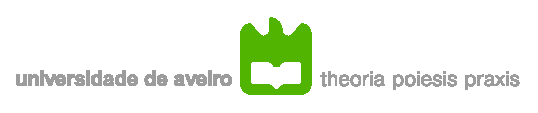
\includegraphics[scale=1]{logo_UA}
\linebreak\linebreak
\LARGE\textbf{Eletricidade \& Magnetismo}
\normalsize\linebreak
(2013-2014)
\linebreak\linebreak
\textbf{Relat\'{o}rio Individual de Laborat\'{o}rio}
\linebreak
10 de dezembro de 2013
\linebreak\linebreak
\underline{Vers\~{a}o B}
\end{center}

\noindent\textcolor{red}{\textbf{Aten\c{c}\~{a}o! Deve indicar a versão da prova na folha de resposta.}}


~\linebreak
\noindent\textbf{Nome:}~\underline{\hspace{9cm}}~\textbf{Nº Mecanogr\'{a}fico:}~\underline{\hspace{2.5cm}}

~\linebreak
\noindent\textbf{Justifique todas as respostas!}

~\linebreak
\noindent\textbf{1) Eletroest\'{a}tica} \hfill [\textit{3 valores}]

Um aluno eletriza uma barra de PVC e aproxima-a da cabe\c{c}a do eletrosc\'{o}pio de folha, at\'{e} finalmente a tocar com a ponta da barra. Explique o que acontece ao longo do processo experimental, explicitando todos os fluxos de carga relevantes. Diga tamb\'{e}m, justificando, se a experi\^{e}ncia lhe permite determinar o sinal da carga na barra.

~\linebreak
\noindent\textbf{2) Circuitos de corrente cont\'{i}nua} \hfill [\textit{2 valores}]

Determine o circuito equivalente de Th\'{e}venin \`{a} esquerda dos nodos A e B do circuito esquematizado na Fig.~\ref{fig:thevenin}.

\begin{figure}[h]
\begin{center}
\begin{pspicture}[showgrid=false](9,4)
\pnode(1,0){A}
\pnode(4,0){B}
\pnode(7,0){C}
\pnode(1,3){D}
\pnode(4,3){E}
\pnode(5,0){F}
\pnode(5,3){G}
\pnode(8,3){a}
\pnode(8,0){b}
\vdc[labeloffset=-1.4](D)(A){$15.0~\text{V}$}
\resistor[dipolestyle=zigzag](D)(E){$1\text{k}5$}
\resistor[dipolestyle=zigzag](B)(E){$220$}
\resistor[dipolestyle=zigzag](G)(F){$2\text{k}2$}
\resistor[dipolestyle=zigzag,arrows=-o](G)(a){$470$}
\wire[arrows=*-*](E)(G)
\wire[arrows=*-*](B)(F)
\wire[arrows=*-o](F)(b)
\wire(B)(A)
\uput[r](a){$A$}
\uput[r](b){$B$}
\end{pspicture}
\end{center}
\caption{\label{fig:thevenin}Circuito a simplificar.}
\end{figure}

~\linebreak
\noindent\textbf{3) Bobinas de Helmholtz} %\hfill [\textit{7,5 valores}]

Recorde o trabalho sobre o estudo do campo magn\'{e}tico produzido pelas bobinas de Helmholtz.

\textbf{a)} \hfill [\textit{3 valores}]

Durante a realiza\c{c}\~{a}o deste trabalho experimental mediu o campo magn\'{e}tico por meio de uma sonda de efeito de Hall. Explique e esquematize o que \'{e} o efeito de Hall num semicondutor. Assuma que os portadores de carga maiorit\'{a}rios t\^{e}m carga positiva.

\textbf{b)} \hfill [\textit{2,5 valores}]

A calibra\c{c}\~{a}o da sonda de efeito de Hall foi feita recorrendo a um solenoide padr\~{a}o com $3467\pm60$ espiras por metro. As medidas obtidas est\~{a}o presentes na Tabela~\ref{tab:hall}. Com base nestes valores, obtenha a constante de calibração da sonda, bem como a respetiva incerteza e represente graficamente a tens\~{a}o de Hall ($V_H$) em fun\c{c}\~{a}o do m\'{o}dulo do campo magn\'{e}tico no interior do solenoide ($B_S$). O campo magn\'{e}tico ao longo do eixo de um solenoide infinito \'{e} dado pela Eq.~\ref{eq:solenoide}.
\begin{equation}
\label{eq:solenoide}
\left|\overrightarrow{B_S}\right|=\mu_0\frac{N}{l}I_S
\end{equation}

\begin{table}[h]
\caption{\label{tab:hall}Tens\~{a}o ($V_H$) amplificada da sonda por efeito de Hall em fun\c{c}\~{a}o da corrente ($I_S$) que atravessa o solenoide padr\~{a}o.}
\begin{center}
\begin{tabular}{|c|c|}
\hline
$I_S~\pm~0,01$ (A) & $V_H~\pm~1$ (mV) \\ \hline
0,08 & 9 \\ 
0,09 & 10 \\ 
0,11 & 11 \\ 
0,12 & 13 \\ 
0,14 & 15 \\ 
0,18 & 19 \\ 
0,25 & 28 \\ 
0,32 & 35 \\ 
0,48 & 54 \\ 
0,77 & 86 \\ 
1,00 & 114 \\ \hline
\end{tabular}
\end{center}
\end{table}

\textbf{c)} \hfill [\textit{2 valores}]

Para \underline{uma bobina} colocou-se a sonda de efeito de Hall no centro da mesma tendo sido medido o valor de $V_H\pm\Delta V_H=50\pm1~\text{mV}$. Sabendo que a corrente que atravessa a bobina é $I\pm\Delta I=0.50\pm0.01~\text{A}$, o raio da bobina é de $R\pm\Delta R=3.5	\pm0.1~\text{cm}$ e que a norma do campo magn\'{e}tico no eixo de uma espira ao longo do seu eixo \'{e} dado pela Eq.~\ref{eq:anel}, determine o n\'{u}mero de espiras na bobina, bem como a incerteza associada.
\begin{equation}
\label{eq:anel}
B\left(x\right)=\frac{\mu_0}{2}\frac{IR^2}{\left(R^2+x^2\right)^{3/2}}
\end{equation}

~\linebreak
\noindent\textbf{4) Indu\c{c}\~{a}o} %\hfill [\textit{7,5 valores}]

Recorde o trabalho sobre a Indu\c{c}\~{a}o que consistiu na varia\c{c}\~{a}o do fluxo magn\'{e}tico por varia\c{c}\~{a}o da corrente que flui numa bobina.

\textbf{a)} \hfill [\textit{2,5 valores}]

Considere um circuito no qual est\~{a}o ligados em s\'{e}rie um gerador de sinal, uma resist\^{e}ncia de $R\pm\Delta R=100\pm5~\Omega$ e um solenoide (daqui em diante referido como \emph{prim\'{a}rio}) de raio $r\pm\Delta r=1.38\pm0.01~\text{cm}$ e $N/l\pm\Delta N/l=3000\pm15$ espiras por metro. Uma bobina (daqui em diante referida como \emph{secund\'{a}rio}) de $N_b\pm\Delta N_b=1200\pm6$ espiras envolve o \emph{prim\'{a}rio}. Aplica-se um sinal triangular ao circuito \emph{prim\'{a}rio} tendo-se observado nos terminais da resist\^{e}ncia o sinal do Canal A da Fig.~\ref{fig:osci1}. O sinal induzido no \emph{secund\'{a}rio} é o que se observa no Canal B da mesma figura.

Determine o coeficiente de indu\c{c}\~{a}o m\'{u}tua observado e compare-o com o esperado, sabendo que a for\c{c}a eletromotriz (f.e.m.) induzida no \emph{secund\'{a}rio} é dada pela Eq.~\ref{eq:fem}.

\begin{equation}
\label{eq:fem}
\varepsilon=\pi\mu_0\frac{N}{l}r^2N_b\frac{\mathrm d i}{\mathrm d t}
\end{equation}

\textbf{b)} \hfill [\textit{2,5 valores}]

Nas condi\c{c}\~{o}es experimentais da al\'{i}nea \textbf{a)}, alterou-se a forma do sinal, aplicando-se ao \emph{prim\'{a}rio} um sinal tipo "dente-de-serra", como mostra o Canal A da Fig.~\ref{fig:osci2}. Esboce a forma do sinal que espera obter no \emph{secund\'{a}rio}. \underline{Justifique a sua escolha}.

\textbf{c)} \hfill [\textit{2,5 valores}]

Nas condi\c{c}\~{o}es experimentais da al\'{i}nea \textbf{a)}, introduziu-se uma barra de ferrite no interior das bobinas e aplicou-se ao \emph{prim\'{a}rio} o mesmo sinal do Canal A da Fig.~\ref{fig:osci1}. Qual \'{e} agora a amplitude da f.e.m induzida no \emph{secund\'{a}rio}, assumindo que $\mu_\text{Ferrite}=8.0\times10^{-4}$ H/m é um valor exato.

\begin{figure}[h]
\begin{center}
\newpsstyle{Dash}{linestyle=dashed,
linecolor=black,linewidth=0.035,plotpoints=50}
\psscalebox{1}{
\Oscillo[Wave1=\TriangleA,
         Wave2=\RectangleB,
    amplitude1=4.00,
    amplitude2=-0.3,
       period1=1.2,
       period2=1.2,
        phase1=0.0,
        phase2=0.0,        
    sensivity1=1.0,
    sensivity2=0.2,
       timediv=0.15,
       offset2=0.9,        
    plotstyle1=Dash,
      AllColor=false]}
\caption{\label{fig:osci1}Visor do oscilosc\'{o}pio. O Canal A est\'{a} representado a tracejado enquanto o Canal B a cheio.}
\end{center}
\end{figure}

\begin{figure}[h]
\begin{center}
\newpsstyle{Dash}{linestyle=dashed,
linecolor=black,linewidth=0.035,plotpoints=50}
\psscalebox{1}{
\Oscillo[Wave1=\LDogToothA,
    amplitude1=0.25,
       period1=0.27,
    sensivity1=0.1,
         Wave2=\RectangleB,
    amplitude2=0,
       period2=0.38,
        phase2=90,
    sensivity2=0.02,
           CC2=10,
       timediv=0.05,
      AllColor=false]}
\caption{\label{fig:osci2}Visor do oscilosc\'{o}pio mostrando apenas o Canal A, representado a cheio.}
\end{center}
\end{figure}

\cleardoublepage

\noindent\textbf{Constantes:}

\noindent$\mu_0=4\pi\times10^{-7}$ (H/m) [valor exato]

\noindent\textbf{Incerteza:}

\noindent$G \equiv f\left(x_1,x_2,\dotsc,x_n\right)$,

\begin{equation*}
\Delta G = \sqrt{\sum_{i=1}^{n}{\left(\frac{\partial G}{\partial x_i}\Delta x_i\right)^2}}
\end{equation*}


\end{document}